\documentclass[12pt,a4paper,titlepage]{article}
\usepackage[utf8x]{inputenc} 
\usepackage[ngerman]{babel}
\usepackage{a4wide}
\usepackage{graphicx}
\author{Otto Ritter\\me@otto-ritter.de}
\title{Spezielle Algorithmen}
\begin{document}
\bibliographystyle{plain}
\begin{titlepage} 
\begin{center}
\begin{Huge}
IT-Sicherheit\\
\end{Huge}
\vspace*{0,5cm}
\begin{Large}
Ausarbeitung\\
\end{Large}
\vspace*{1,2cm}
Autor: Otto Ritter\\
Matrikelnummer: 10012669\\
eMail: me@otto-ritter.de\\
\vspace{1cm}
13.02.2012
\end{center}
\end{titlepage}
\newpage
\tableofcontents
\thispagestyle{empty}
\nocite{*}
\newpage
\setcounter{page}{1}
\section{Einleitung}
\subsection{Ausgangslage}
Es soll ein Programm entwickelt werden, dass dazu dient, Dateien sicher und einfach mit Freunden und Bekannten zu teilen. Dabei sollen die zu übertragenden Dateien unter hohen Sicherheitsaspekten so verschlüsselt werden, dass kein Dritter Zugriff erlangt.
\subsection{Vorüberlegung}
Das Programm soll möglichst selbsterklärend, schlicht und sicher sein. Die grafische Oberfläche soll so wenige Elemente wie möglich haben, um den Benutzer nicht unnötig zu belasten.
\subsection{Verwendete Software}
Das Programm wurde mit C++ und Qt\footnote{Ein Bibliothek für C++ das von Nokia gepflegt wird.} geschrieben. Für kryptografische Verfahren wurde OpenSSL\footnote{Eine Bibliothek die viele gängigen Verschlüsselung verfahren enthält.} eingesetzt.
\section{Lösungsansätze}
\subsection{Geschwindigkeit}
Damit das Programm auch bei größeren Dateien nicht zu lange braucht, kommen nur die symmetrischen\footnote{Benutzt den selben Schlüssel zu Ver- und Entschlüsseln.} Algorithmen in Frage. Hier entsteht das Problem wie der Schlüssel für die symmetrische Verschlüsselung übertragen wird. Die Lösung besteht in asymmetrischen\footnote{Zum Ver- und Entschlüsseln werden verschiedene Schlüssel verwendet} Algorithmen. 
\subsection{Schlüssel}
Eine Schwachstelle ist meist der Benutzer, der oft den selben Schlüssel mehrfach verwendet. Zudem ist dieser oft kurz oder leicht zu erraten, denn es wird oft das Geburtsdatum oder ähnliches gewählt. Um die Schwachstelle umgehen zu können, sollte der Schlüssel zufällig erzeugt werden. Wie schon erwähnt, muss der erzeugte Schlüssel an den Empfänger weitergegeben werden, ohne dass Dritte diesen abgreifen können. Hierzu sollen asymmetrische Algorithmen eingesetzt werden, um den erzeugten Schlüssel zu verschlüsseln. Eines der asymmetrischen Algorithmen ist RSA, das erzeugte Schlüsselpaar ist mathematisch voneinander abhängig. Das, was mit dem öffentlichen Schlüssel verschlüsselt wurde, kann mit dem privaten wieder entschlüsselt werden. Das bedeutet, dass der symmetrische Schlüssel mit dem öffentlichen RSA-Schlüssel des Empfängers verschlüsselt wird, dieser kann ihn dann mit dem privaten Schlüssel öffnen. Somit muss vor jedem Verschlüsseln der öffentliche Schlüssel des Empfängers bekannt sein. Um das Programm benutzerfreundlich zu gestalten, sollte eine Schlüsselverwaltung implementiert werden. Ich habe mich dazu entschieden, eine Kontaktliste zu implementieren, denn viele Nutzer kennen solche Listen bereits aus anderen Echtzeit-Kommunikationsprogrammen. Die öffentlichen Schlüssel werden lokal auf dem Computer gespeichert.
\subsection{Freunde}
Ein Eintrag in der Freundesliste beinhaltet die Bezeichnung des Empfängers und seines öffentlichen Schlüssels. Als Bezeichnung des Empfängers kann der Name oder die E-Mail Adresse benutzt werden. Es soll darauf geachtet werden, dass die Bezeichnung einzigartig bleibt. Die Liste bietet nur die drei wichtigsten Operationen: Anlegen, Bearbeiten und Löschen.
\newpage
\section{Technische Umsetzung}
\subsection{Klassen}
\begin{figure}[ht]
  \centering
  \fbox{ 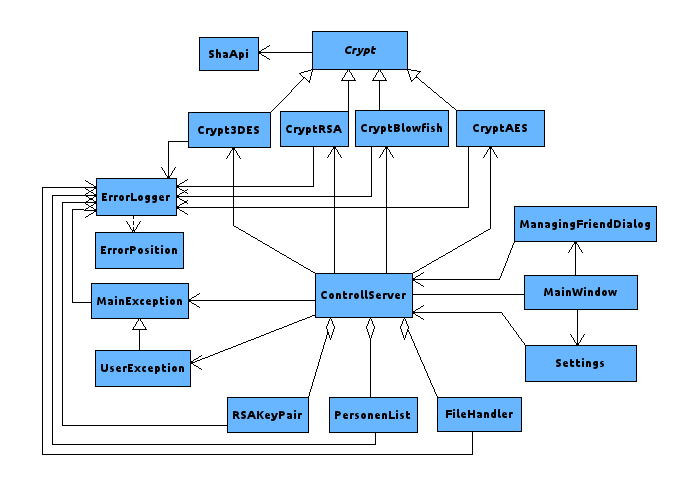
\includegraphics[scale=0.8]{Klassendiagramm.png} }
  \caption{Klassen Hierarchie}
  \label{class_digram}
\end{figure}
\begin{description}
	\item[MainWindow] Beinhaltet die grafischen Elemente, also das View (Abbildung \ref{t3_mainwindow}).
	\item[ManagingFriendDialog] ist der Dialog für die Freunde Verwaltung. (Abbildung \ref{t3_addfriendwindow} und \ref{t3_editfriendwindow})
	\item[Settings] Der Dialog für die Einstellungen. (Abbildung \ref{t3_settingswindow})
	\item[ControllServer] Der Controller des Programms ist ein Singleton und bildet die Schnittstelle zwischen grafischer Oberfläche und Programmlogik bzw. Datenhaltung.
    \item[Crypt]  Die Basisklasse für alle Verschlüsselungs-Klassen.
    \item[Crypt3DES] Wrapper für die 3DES Implementierung zum verschlüsseln der Daten. Ist sicher aber langsam.
    \item[CryptAES] Wrapper für die AES Implementierung zum verschlüsseln der Daten. Ist der Nachfolger des DES und schneller als dieser.
    \item[CryptBlowfish] Wrapper für die Blowfish Implementierung zum verschlüsseln der Daten. Schneller Algorithmus.
    \item[CryptRSA] Wrapper für die RSA Implementierung zum verschlüsseln von Daten. Asymmetrische Algorithmus.
    \item[ShaApi] Wrapper für die SHA1 und SHA2 Familie.
    \item[FileHandler] Ist für das einlesen und schreiben der Dateien auf die Festplatte zuständig.
    \item[ErrorLogger] Singleton zum schreiben in die Logdatei.
    \item[ErrorPosition] Bestimmt mit Preprozessor Direktiven an welcher Stelle im Code der der Aufruf erfolgte. Wichtig zum finden von Fehlern.
    \item[MainException] Ist von std::exception abgeleitet und enthält nur die technische Nachrichten.
    \item[UserException] Ist von MainException abgeleitet und enthält die technische und Benutzerfreundliche Nachrichten.    
    \item[PersonenList] Datenhaltungs-Klasse für die Freundes-liste
    \item[RSAKeyPair] Verwaltet das eigene Schlüsselpaar für das RSA verfahren.
  \end{description}
\subsection{Verschlüsselungen}
Von der Basisklasse Crypt werden die übrigen Klassen abgeleitet. Die Basisklasse definiert eine Schnittstelle, welche die virtuellen Methoden encrypt und decrypt beinhaltet. Da die RSA-Verschlüsselung mit zwei Schlüsseln umgehen muss, bekommt diese weitere Methoden. Ebenso wurde eine weitere Klasse zur Bildung von Prüfsummen, nach dem SHA1, SHA256 und SHA512 Algorithmen, implementiert.
Die Basisklasse besitzt zudem Methoden, um zufällige Zeichenfolgen zu erzeugen.Dabei wird auf Linux Systemen von /dev/urandom eingelesen. Auf Windows-Systemen wird die Uhrzeit eingelesen. Aus der eingelesenen Zeichenkette wird mit dem SHA512 Algorithmus eine Prüfsumme gebildet, davon wird die gewünschte Länge abgeschnitten und zurückgegeben.
\subsection{Datenhaltung}
Es gibt zwei Klassen für die Datenhaltung, die Freundesliste und die Schlüsselpaare. Beide Klassen laden und speichern ihre Einträge, beim schließen und öffnen des Programms, eigenständig im XML-Format.
\subsection{Der Controller}
Die Klasse ControllServer bildet den Controller. Der Controller hat Zugriff auf die Verschlüsselungsklassen, Datenhaltungslassen, Hilfsklassen und die grafische Oberfläche und bildet damit eine Schicht zwischen Frontend und Backend. Er fängt die Ausnahmen und gibt nur die für den Benutzer relevanten Fehler und Warnungen an die GUI\footnote{Graphical User Interface - grafische Benutzeroberfläche} weiter.
\subsection{Die Helfer}
Die Klasse ErrorLogger wurde implementiert um Logdatein zu schreiben. Diese Datei enthält Fehler, Warnungen und Informationen. Es stehen zwei Klassen für Behandlungen von Ausnahmen zur Verfügung. Die Klasse MainException sollte für Fehlerbehandelung benutzt werden, die UserException sollte dafür benutzt werden um dem Nutzer Fehler mitzuteilen. Diese erzeugt intern eine MainException, um für den Entwickler einen Eintrag in der Logdatei zu erfassen. Es ist natürlich möglich, mit der MainException auszukommen, doch wird so ein bessere Trennung zwischen technischen und nicht technischen Ausnahmen gemacht. Die MainExceptions benutzen den ErrorLogger, um die Fehler in die Datei zu schreiben.
\newpage
\subsection{Funktionsablauf}
\subsubsection{Verschlüsseln}
\begin{figure}[ht]
  \centering
  \fbox{ 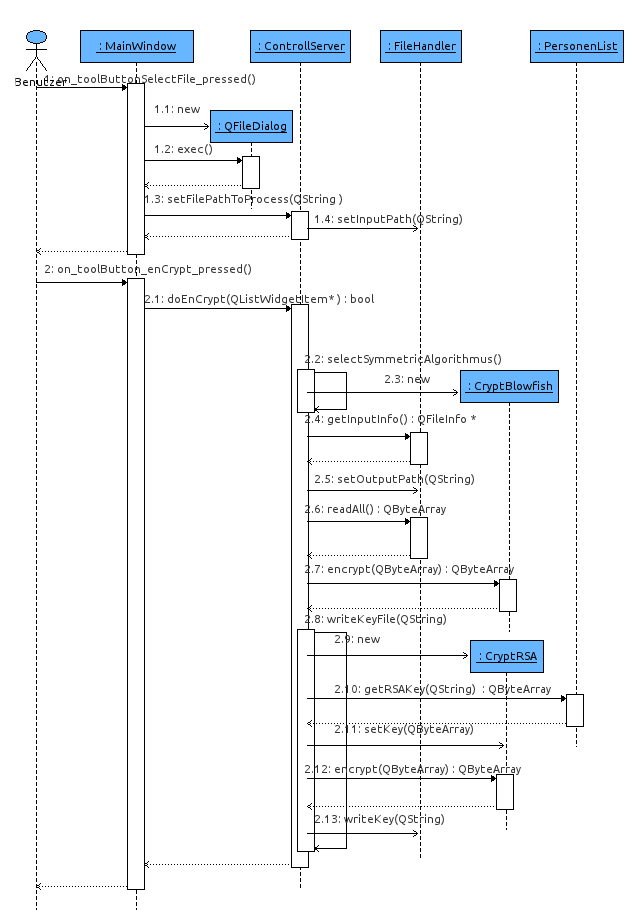
\includegraphics[scale=0.55]{Seq_Verschluesseln.png} }
  \caption{Sequenzdiagramm Verschlüsseln}
  \label{seq_diagramencrypt}
\end{figure}
Wenn der Benutzer eine Datei und den Empfänger gewählt hat, kann er die Verschlüsselung starten. Nachdem der Controller ein Crypt-Objekt des gewählten symmetrischen Algorithmus erzeugt hat, wir die ausgewählte Datei eingelesen und zur Verschlüsselung weitergegeben. Alle symmetrischen Algorithmen\\ erzeugen einen zufälligen Initialisierungsvektor und einen optimalen Schlüssel für den gewählten Algorithmus. Wenn die Verschlüsselung erfolgreich war, wird der Initialisierungsvektor vor die verschlüsselten Daten geschrieben und zurückgegeben. Der Controller leitet diese Daten an den FileHandler weiter, dieser schreibt sie auf die Festplatte. Bei Fehlern werden Ausnahmen geworfen die der Controller fängt und von ihm verarbeitet werden. Der Controller erzeugt für die verschlüsselte Datei nun eine key-Datei, worin der symmetrische Schlüssel mit dem RSA-Algorithmus und dem öffentlichen Schlüssel des Empfängers verschlüsselt wird. Beim Schreiben in die Schlüsseldatei werden von den Werten Checksummen mit dem MD5 Algorithmus gebildet und mit dazu geschrieben, damit der Empfänger prüfen kann ob die Schlüsseldatei unbeschadet angekommen ist. Wenn alles fehlerfrei abgelaufen ist, wird die Status-Anzeige auf 100\% gesetzt.
\subsubsection{Entschlüsseln}
\begin{figure}[ht]
  \centering
  \fbox{ 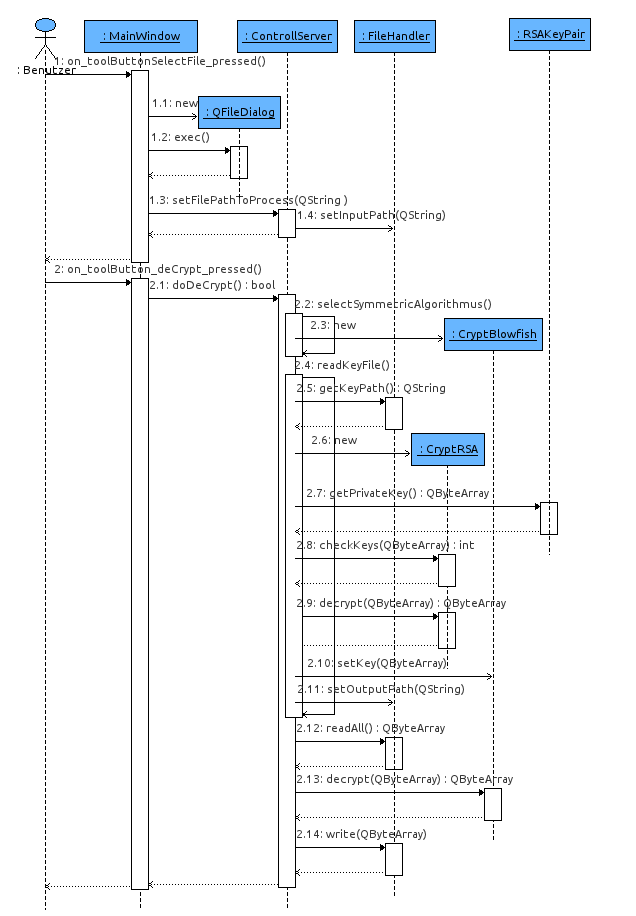
\includegraphics[scale=0.6]{Seq_Entschluesseln.png} }
  \caption{Sequenzdiagramm Entschlüsseln}
  \label{seq_diagramdecrypt}
\end{figure}

Nach dem Auswählen der Schlüsseldatei oder einer verschlüsselten Datei kann durch den Benutzer die Entschlüsselung eingeleitet werden. Die GUI ruft die entsprechende Methode im Controller auf, dieser liest die Schlüsseldatei ein und prüft ob die Checksumme übereinstimmen. Nun wird noch geprüft ob der öffentliche Schlüssel zum eigenen privaten Schlüssel passt. Wenn der öffentliche Schlüssel passt, wird der symmetrische Schlüssel wieder mit dem RSA-Algorithmus entschlüsselt, dazu wird der eigene private Schlüssel verwendet. Nachdem der symmetrische Schlüssel zur Verfügung steht wird mit der symmetrischen Entschlüsselung fortgefahren. Dazu wird wieder das Objekt mit dem gewählten symmetrischen Algorithmus erzeugt und der symmetrische Schlüssel gesetzt. Der FileHandler liest die Datei ein, diese wird über den Controller zur Verschlüsselung weitergereicht. Das Objekt, dass für Ver- und Entschlüsselung zuständig ist, liest den Initialisierungsvektor ein und startet die Entschlüsselung. Wenn keine Fehler aufgetreten sind, werden die Daten wieder an den Controller übergeben und auf die Festplatte geschrieben sowie die Status-Anzeige auf 100\% gesetzt.
\newpage
\section{T³ - Trusted Transmission Tool}
\subsection{Übersicht}
\begin{figure}[ht]
  \centering
  \fbox{ 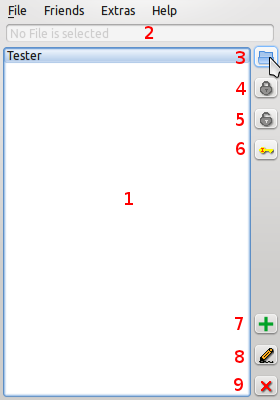
\includegraphics[scale=0.9]{MainWindow.png} }
  \caption{T³ Hauptfenster}
  \label{t3_mainwindow}
\end{figure}
\begin{enumerate}
\item Liste der Freunde.
\item Zeigt die ausgewählte Datei an, die verschlüsselt oder entschlüsselt werden soll.
\item Öffnet einen Dialog zum auswählen einer Datei.
\item Um die gewählte Datei zu verschlüsseln.
\item Um die gewählte Datei zu entschlüsseln.
\item Kopiert den öffentlichen Schlüssel in die Zwischenablage und exportiert diesen als myPublic.key Datei am selben Ort, wo das ausführbare Programm liegt.
\item Öffnet einen Dialog zum hinzufügen neuer Freunde.
\item Öffnet einen Dialog zum bearbeiten vorhandener Freunde.
\item Löscht einen vorhandenen Freund.
\end{enumerate}
\begin{figure}[ht]
  \centering
  \fbox{ 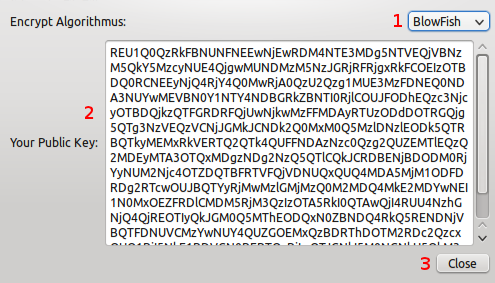
\includegraphics[scale=1]{SettingsWindow.png} }
  \caption{T³ Einstellungen}
  \label{t3_settingswindow}
\end{figure}
\begin{enumerate}
\item Auswahl des symmetrischen Verschlüsselungsalgorithmus.
\item Anzeige des eigenen öffentlichen Schlüssels ( Änderung ist nicht möglich ).
\item Zum Schließen des Dialoges.
\end{enumerate}
\newpage
\begin{figure}[ht]
  \centering
  \fbox{ 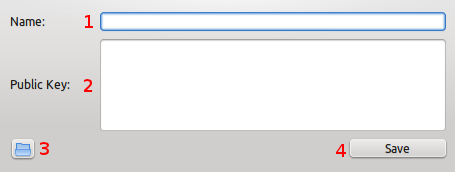
\includegraphics[scale=1]{AddFriendWindow.png} }
  \caption{T³ Freund hinzufügen}
  \label{t3_addfriendwindow}
\end{figure}
\begin{enumerate}
\item Eingabefeld für die Bezeichnung des Empfängers.
\item Eingabefeld für den öffentlichen Schlüssel des Empfängers.
\item Schaltfläche zum Laden des öffentlichen Schlüssel aus einer Datei.
\item Schaltfläche zum Speichern der Eingaben, um einen Empfänger anzulegen und zum schließen des Dialoges.
\end{enumerate}
\begin{figure}[ht]
  \centering
  \fbox{ 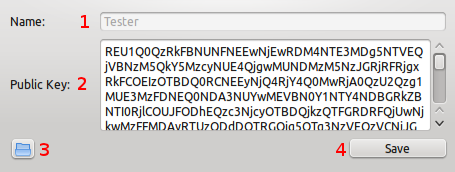
\includegraphics[scale=1]{EditFriendWindow.png} }
  \caption{T³ Freund bearbeiten}
  \label{t3_editfriendwindow}
\end{figure}
\begin{enumerate}
\item Eingabefeld für die Bezeichnung des Empfängers. ( Änderung ist nicht möglich ).
\item Eingabefeld für den öffentliche Schlüssel des Empfängers.
\item Schaltfläche zum laden des öffentlichen Schlüssel aus einer Datei.
\item Schaltfläche zum Speichern der Änderungen eines Empfängers und zum schließen des Dialoges.
\end{enumerate}
\newpage
\subsection{Bedienungsanleitung}
\subsubsection{Freund hinzufügen}
Um ein neuen Freund hinzuzufügen kann mit Betätigen des Hinzufügen-Knopfes (7) oder einem Klick im Menü Friends->Add der entsprechende Dialog ( siehe Abbildung \ref{t3_addfriendwindow} ) geöffnet werden. Hierfür muss der öffentliche Schlüssel des Empfängers bekannt sein.
Vorsicht: Bei Eingabe eines schon vorhandenen Namens wird der alte Freund überschrieben. 
\subsubsection{Freund bearbeiten}
Zuerst muss der Freund, der bearbeitet werden soll, in der Liste ausgewählt werden. Dann auf den Bearbeiten-Knopf (8) oder im Menü Friends->Edit klicken. Es erscheint ein Dialog ( siehe Abbildung \ref{t3_editfriendwindow} ) mit den aktuell gespeicherten Angaben. Hier ist es nun möglich, einen anderen Schlüssel einzugeben.
\subsubsection{Freund löschen}
Zuerst muss der Freund, der bearbeitet werden soll, in der Liste ausgewählt werden. Dann auf den Löschen-Knopf klicken (9). Nach dem Bestätigen dieser Aktion wird der Freund gelöscht.
\subsubsection{Verschlüsseln}
Der Benutzer wählt einen vorhanden Empfänger aus der Liste und die Datei, die er Verschlüsseln möchte. Die Datei kann mit der Schaltfläche 3, wie in Abbildung \ref{t3_mainwindow} dargestellt, gewählt werden. Mit dem Betätigen der Schaltfläche 4, zu sehen in der Abbildung \ref{t3_mainwindow}, wird mit der Verschlüsselung begonnen. Nach Abschluss der Verschlüsselung sollten sich zwei weitere Dateien im Ausgewähltem Verzeichnis befinden. Diese werden nach dem Muster Empfängerbezeichnung\_Dateiname.enc und Empfängerbezeichnung\_Dateiname.key, erzeugt. Der Empfänger benötigt beide Dateien zum Entschlüsseln.
\subsubsection{Entschlüsseln}
Der Benutzer wählt mit der Schaltfläche 3 im Hauptfenster die zu entschlüsselnde Datei aus. Dabei ist es irrelevant, ob die gewählte Datei eine .enc oder .key Endung hat. Mit dem Betätigen der Schaltfläche 5 im Hautfenster (siehe Abbildung \ref{t3_mainwindow}) wird mit der Entschlüsselung begonnen. Sobald die Entschlüsselung abgeschlossen ist, befindet sich die entschlüsselte Datei im selben Verzeichnis, in dem die verschlüsselte Datei ausgewählt wurde.
\subsubsection{Hilfe}
Das Programm bietet die Möglichkeit ein Userguide zu öffnen, dieses ist im Menü Help untergebracht. Der Eintrag Userguide öffnet dabei den Standard Webbrowser des Benutzer mit der Adresse http://t3.otto-ritter.de. 
\addcontentsline{toc}{section}{Literatur}
\bibliography{ITS2011_OttoRitter}
\end{document}